\chapter{Planificación}
\title{Planificación}
\label{cap:Planificacion}

Este proyecto se ha planificado siguiendo los puntos que a continuación se detallan y que permiten trabajarlo de una manera ordenada a la vez que dan información al lector facilitándole una visión amplia y exhaustiva, así como la comprensión de la posterior exposición del mismo. A continuación se detallan los diferentes puntos de la planificación que han sido estudiados para este proyecto

\section{Metodología de Desarrollo}
La metodología utilizada ha sido el modelo de desarrollo de prototipos iterativo que es el que más y mejor se ajusta a las características del proyecto. La elección de este tipo de metodología se justifica por los siguientes aspectos de la misma:

\begin{itemize}
  \item Permite un entendimiento incremental del proyecto.
  \item Habilita una fácil retroalimentación al usuario.
  \item Dispone de objetivos parciales y metas concretas.
  \item El proceso es medido conforme avanzan todas las implementaciones.
\end{itemize}

\begin{figure}[htb]
\centering
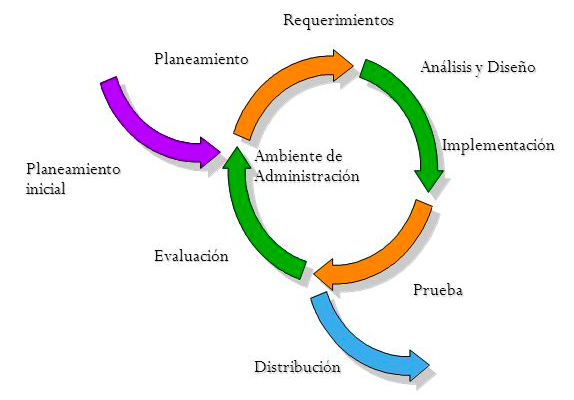
\includegraphics[width=1\textwidth]{./imagenes/modeloIterativo}
\caption{Modelo Iterativo (http://adsi.foroactivo.com//)} \label{fig:modeloIterativo}
\end{figure}

Además de la utilización del modelo iterativo que por sus características específicas es el más idóneo para este trabajo, hay que mencionar que para el control de versiones del proyecto se ha estado utilizando el software Git y para guardar los datos se ha recurrido al servicio GitHub.

\section{Fases}
En este punto se van a exponer de manera más exhaustiva y se va a entrar en detalle, cada una de las fases que se desarrollan para completar el proyecto viéndose, de esta forma, el progreso del mismo.

\subsection{Planteamiento del Problema}
\begin{itemize}
  \item Descripción: Exposición del problema que se desea resolver, pautas a seguir y familiarización con las tecnologías.
  \item Apartado: Capítulo \ref{cap:Introduccion}.\\
\end{itemize}

\subsection{Especificaciones del Proyecto}
\begin{itemize}
  \item Descripción: Obtención de los requisitos funcionales y requisitos no funcionales del proyecto.
  \item Apartado: Capítulo \ref{cap:Analisis}.\\
\end{itemize}

\subsection{Planificación}
\begin{itemize}
  \item Descripción: Estimación temporal, estimación de costes económicos y estimación de recursos humanos.
  \item Apartado: Capítulo \ref{cap:Planificacion}.\\
\end{itemize}

\subsection{Ingeniería}
\begin{itemize}
  \item Descripción: Análisis de los requisitos y diseño del sistema a desarrollar.
  \item Apartado: Capítulos \ref{cap:Analisis} y \ref{cap:DisenoEImplementacion}.\\
\end{itemize}

\subsection{Construcción}
\begin{itemize}
  \item Descripción: Implementación del proyecto.
  \item Apartado: Capítulo \ref{cap:DisenoEImplementacion}.\\
\end{itemize}

\subsection{Pruebas}
\begin{itemize}
  \item Descripción: Pruebas internas del proyecto
  \item Apartado: Capítulo \ref{cap:Pruebas}.\\
\end{itemize}


\section{Estimación Temporal}
Seguidamente se hace una estimación temporal del proyecto detallando cada una de las fases de la sección anterior.

\begin{itemize}
  \item \textbf{Planteamiento del Problema:}
  \begin{itemize}
    \item Descripción de los objetivos a grandes rasgos.
    \item Comprender el protocolo INDI.
    \item Entender los diferentes instrumentos que intervendrán en el protocolo.
    \item Planteamiento de las posibles tecnologías que se usarán en el proyecto.
  \end{itemize}
\end{itemize}
\textit{\textbf{Estimación: 20 horas.}}\\ \\

\begin{itemize}
  \item \textbf{Especificaciones del Proyecto:}
  \begin{itemize}
    \item Conocer perfectamente las necesidades del usuario.
    \item Establecer los objetivos que deben plantearse ante este proyecto.
    \item Extracción de los requisitos funcionales.
    \item Extracción de los requisitos no funcionales.
  \end{itemize}
\end{itemize}
\textit{\textbf{Estimación: 30 horas.}}\\ \\

\begin{itemize}
  \item \textbf{Análisis y Diseño:}
  \begin{itemize}
    \item Análisis de los requisitos que debe reunir este proyecto.
    \item Diagramas del proyecto.
    \item Metodología empleada en el desarrollo del proyecto
  \end{itemize}
\end{itemize}
\textit{\textbf{Estimación: 40 horas.}}\\ \\

\begin{itemize}
  \item \textbf{Construcción:}
  \begin{itemize}
    \item Establecimiento de las herramientas, las plataformas, los diferentes tipos de lenguajes y el \textit{software} que se va a utilizar
    \item Creación de la interfaz para conectarse a un servidor INDI concreto mediante su IP y su puerto.
    \item Creación de la interfaz para mostrar en una ventana el dispositivo con sus grupos y sus diferentes propiedades.
    \item Creación de la interfaz para mostrar, en la pantalla, varias ventanas con diferentes dispositivos conectados al servidor simultáneamente.
    \item Posibilidad de cambiar cualquier parámetro de un dispositivo conectado.
    \item Posibilidad de enviar información al servidor con los parámetros que hayan sido modificados.
  \end{itemize}
\end{itemize}
\textit{\textbf{Estimación: 110 horas.}}\\ \\

\begin{itemize}
  \item \textbf{Pruebas:}
  \begin{itemize}
    \item Pruebas de integración.
    \item Pruebas de sistema.
    \item Pruebas de aceptación.
  \end{itemize}
\end{itemize}
\textit{\textbf{Estimación: 10 horas.}}\\ \\


\begin{itemize}
  \item \textbf{Documentación:}
  \begin{itemize}
    \item Documentación del código del prototipo del cliente.
    \item Documentación del proyecto.
    \item Manual de usuario del prototipo.
  \end{itemize}
\end{itemize}
\textit{\textbf{Estimación: 40 horas.}}\\


\begin{table}[h]
\centering
\label{table:tiempoEstimado}
\begin{tabular}{ll}
\hline
{\bf Tarea a realizar}                   & {\bf Tiempo estimado (horas)} \\ \hline
Planteamiento del problema    & 20 horas                            \\
Especificaciones del proyecto & 30 horas                            \\
Análisis y diseño             & 40 horas                            \\
Construcción                  & 110 horas                           \\
Pruebas                       & 10 horas                            \\
Documentación                 & 40 horas                            \\
{\bf Total}                   & {\bf 240 horas}                           \\ \hline
\end{tabular}
\caption{Estimación temporal}
\end{table}


\section{Recursos Humanos}
Gracias a que se ha elegido en la realización y posterior utilización de este proyecto un \textit{Software Libre}, toda persona que tenga unos conocimientos mínimos en programación, astronomía e INDI, que desee realizar una aportación puede hacerlo en el \href{https://github.com/PabloTorrecillas/IndiWebClient}{repositorio del proyecto}.\\
(https://github.com/PabloTorrecillas/IndiWebClient)

El desarrollo del proyecto ha sido realizado por una única persona y, que en este caso, coincide con el autor del presente documento.

Como para la realización del proyecto, desde su inicio hasta la finalización del mismo, se han utilizado unos 4 meses aproximadamente, se podría decir que el proyecto realizado por una única persona supondría un trabajo desarrollado a lo largo de un periodo de cuatro meses. Por el contrario, si se dispusiera de un equipo formado por cuatro personas, se podría obtener un resultado menor en cuanto a tiempo se refiere.
\section{Recursos \textit{Software} Reutilizables}
Los siguientes recursos hacen mención a diferentes desarrollos software creados por otras empresas o por otros desarrolladores.

Como el objetivo fundamental del proyecto es la creación de un prototipo de cliente Web capaz de controlar un observatorio astronómico desde cualquier lugar del planeta donde exista conexión a internet, se tendrán que tener en cuenta durante el desarrollo, todas aquellas herramientas que permitan realizar el prototipo HTML y aquellas bibliotecas de \textit{Software Libre} que se encuentran en internet. Dichas bibliotecas se podrán consultar y utilizar, tanto para añadir funcionalidad al prototipo de cliente, como para realizar los diferentes elementos gráficos del proyecto.

\section{Estimación de Costes Económicos}
En esta sección se va a proceder a la estimación de todos los costes económicos para poder llevar a cabo el proyecto:

\subsection{Licencias \textit{Software}}
Dado que el proyecto se realiza mediante herramientas de desarrollo de \textit{Software Libre} gratuito no es necesario realizar el pago de ninguna licencia \textit{software}.

\subsection{Recursos Humanos}
Representan la totalidad de personas que forman el equipo y que han contribuido al desarrollo y finalización de este proyecto. El tiempo que se ha empleado para este trabajo arroja un total de 240 horas.

Dado que la ley prohíbe de forma expresa a los Colegios de Profesionales para disponer e informar sobre los honorarios, se tomarán como honorarios a percibir el sueldo medio que recibiría un Graduado en Ingeniería Informática. Partiendo de esta premisa, se hará una estimación de que el precio por hora será de unos 18\euro. El resultado final que se obtiene analizando el coste económico del equipo de trabajo, en este proyecto, sería la cantidad de 4320\euro.

\subsection{Material}
Dado que INDI dispone de diferentes simuladores con los que poder realizar todas las pruebas necesarias para comprobar que el prototipo de cliente funciona, el coste total del material ha sido de 0\euro.

Por otra parte, se puede utilizar una cámara \textit{reflex nikon D3200} con un objetivo 18-55mm valorada en 339,99\euro, según Amazon \cite{NikonAmazon}.

Por último, no se le puede restar al material un elemento imprescindible y de vital importancia para este proyecto como es un ordenador. Gracias al ordenador se podrá llevar a cabo la función de programación, documentación del código, buscar información, etcétera. El precio aproximado es de 450\euro.

Como conclusión, en cuanto a la estimación de costes económicos referidos a la realización de este proyecto, obtenemos los siguientes resultados:
\\ \\
\begin{table}[h]
\centering
\label{table:costeEstimado}
\begin{tabular}{ll}
\hline
{\bf Gastos}                   & {\bf Coste Estimado en euros} \\ \hline
Licencias \textit{software}   & 0\euro                             \\
Recursos humanos              & 4320\euro                          \\
Material                      & 790\euro                           \\
{\bf Total}                   & {\bf 5110\euro}                          \\ \hline
\end{tabular}
\caption{Estimación de coste económico}
\end{table}


\section{Temporización}
Se ha elaborado una estimación temporal acorde a las tareas realizadas en la sección de estimación temporal y atendiendo también al número de días. Para mostrarlo de una forma más sencilla, se han creado diagramas de Gantt que corresponden con cada una de las cuatro iteraciones del proyecto.

\begin{figure}[htb]
\centering
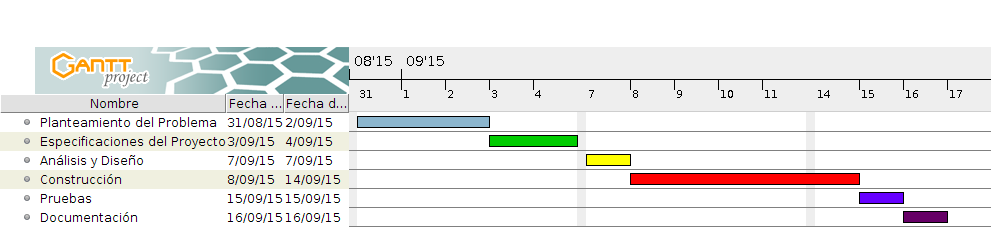
\includegraphics[width=1\textwidth]{./imagenes/iteracion1}
\caption{Iteración 1 de la Planificación} \label{fig:iteracion1}
\end{figure}

\begin{figure}[htb]
\centering
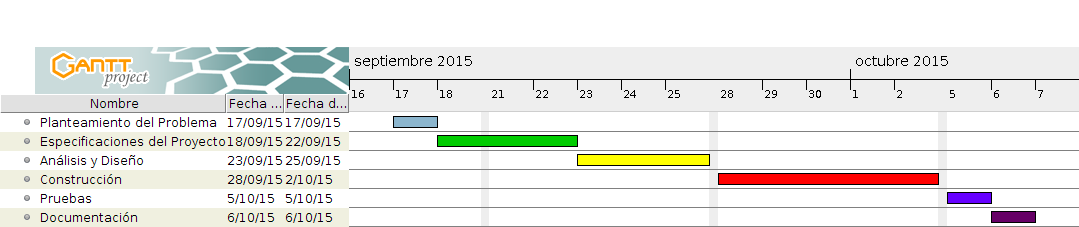
\includegraphics[width=1\textwidth]{./imagenes/iteracion2}
\caption{Iteración 2 de la Planificación} \label{fig:iteracion2}
\end{figure}

\begin{figure}[htb]
\centering
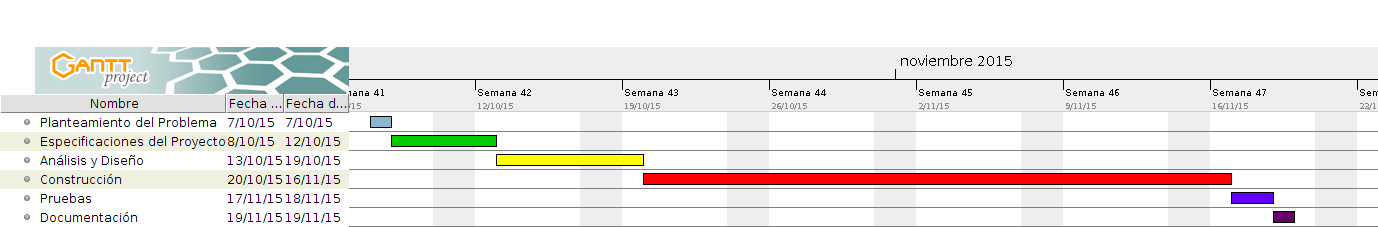
\includegraphics[width=1\textwidth]{./imagenes/iteracion3}
\caption{Iteración 3 de la Planificación} \label{fig:iteracion3}
\end{figure}

\begin{figure}[htb]
\centering
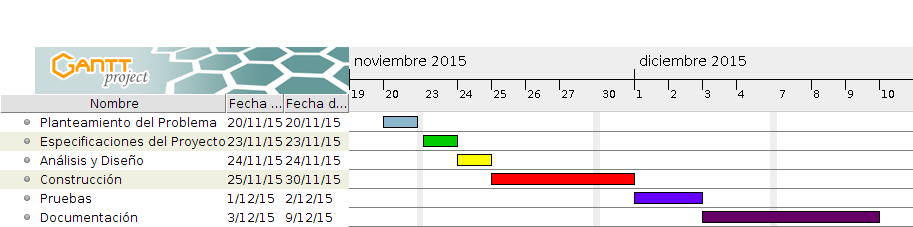
\includegraphics[width=1\textwidth]{./imagenes/iteracion4}
\caption{Iteración 4 de la Planificación} \label{fig:iteracion4}
\end{figure}
